\label{ch:desing}
\chapter{Diseño e Implementación}

\section{Limitaciones técnicas para implementar el prototipo}

\section{Diseño de la solución} 
\subsection{Definición de la política de seguridad}
Detectar si una aplicación Android(perteneciente al conjunto evaluable) presenta
flujos de información entre, información con nivel de seguridad alto e
información con nivel de seguridad bajo.\newline 
Detectando fugas de información catalogada con nivel de seguridad alto, vía:
canales creados durante el control de flujo del programa(flujos implícitos),
mensajes de texto y mensajes de Log.\newline 

\subsection{Consideraciones para verificar el cumplimiento de la política
mediante Jif} 
\textit{Diferencia entre una aplicación Android y una aplicación Java
convencional:}\newline 
En esencia, una aplicación Android es una aplicación Java con interfaces
descritas en XML, que para ser ejecutada necesita del framwork de Android,
porque este le provee acceso al hardware del dispositivo y funcionalidades del
sistema.\newline 
Por otro lado, jif permite hacer seguiemiento al flujo de información de una
aplicación Java, extendiendo el lenguaje mediante labels de seguridad.\newline
Para analizar flujo de información de una aplicación Android mediante
jif, es importante mencionar que mientras una aplicación Java convencional
cuenta con un único método como punto de entrada para inciar su ejecución(el
método main de la clase principal); una aplicación Android puede tener más de un
punto de entrada, generados a partir de los diferentes tipos de componentes que
la pueden integrar(Activity, Service, Content Provider y Broadcast
Receiver). La necesidad de interacción del usuario para activar tales puntos de
entrada varía acorde al tipo de componente, así, en el caso de componentes tipo
Activity su ejecución sólo inicia hasta que el usuario interactue con la
actividad, y para ello cuenta con el método OnCreate. De otro modo, componentes
tipo Service y Broadcast Receiver, inician su ejecución a través de los métodos
OnStartCommand y OnReceive, respectivamente, sin necesidad de interacción del
usuario.\newline 
{ \color{red} {Teniendo en cuenta lo anterior, se asume que la aplicación a
evaluar tiene un único punto de entrada, que depende del tipo de componente que
implemente.} }

\textit{Información considerada con nivel de seguridad alto:}\newline
Para verificar el cumplimiento de la política de seguridad a evaluar se parte de
un conjunto de sources, caracterizados por dar a conocer información del
usuario, considerada como privada o sensible. Los métodos que integran el
conjunto de sources son: getDeviceId, getSimSerialNumber, findViewById,
getLatitude, getLongitude y getSubscriberId. Adicional a estos métodos, se
incluye el campo EditText, si y sólo si, es de tipo textPassword, es decir, un
campo que almacena contraseñas.

\textit{Canales que muestran información con nivel de seguridad bajo}\newline
La información envíada a través de mensajes de texto y la información conocida
tanto a través de mensajes de log, como a través de canales generados por el
control de flujo del programa, tiene en común que debe poder ser conocida por
terceros. En consecuencia, se considera que estos canales deben dar a conocer
información con nivel de seguridad bajo.\newline
En el caso de mensajes de texto y mensajes de log, se hace referencia
específicamente a las clases Log y SmsManager de la API de Android.\newline

\textit{Evaluación del flujo de información:}\newline
Para evaluar el flujo de información, son tenidos en cuenta todos los métodos
definidos dentro de la clase, se asume que todos los métodos son invocados, esto
con el fin de evitar omisiones de flujo de información a través de los canales
previamente mencionados.

\textit{Pasos para el diseño de la solución:}\newline

\begin{figure}[h!]
	\begin{center}
	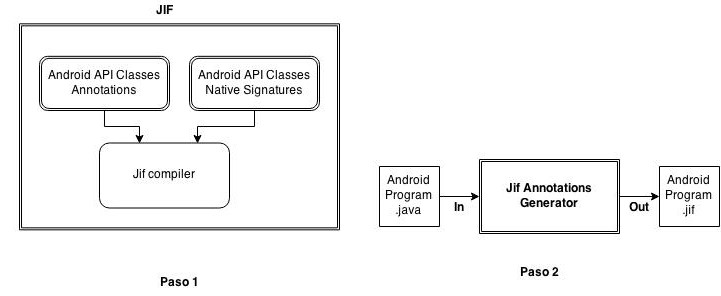
\includegraphics[width=12cm]{desingSol-steps1-2.jpg}
	\end{center}
	\caption{Pasos para el diseño de la solución.}
	\label{fig:desingSol-steps1-2}
\end{figure}

Paso uno: hacer que jif reconozca determinadas clases de la Api de
Android.\newline 
Adicional al mecanismo de anotación que se maneja en jif, en que para hacer
análisis al flujo de información de un programa java, se debe implementar la
versión del respectivo programa para jif. También es posible adicionar clases
Java ya existentes, utilizando signaturas nativas para que el compilador jif las
reconozca, esto es: generando una versión jif de la clase java, donde se
declaran constructores y cuerpo de los métodos a utilizar de la clase fuente
java.\newline
Para el presente trabajo se utilzan ambas opciones de anotación. El criterio
para decidir que se anota de una u otra forma, depende de lo que represente la
clase Android para verificar la política de seguridad establecida. Así, clases
como Activity, BroadcastReceiver y Service, que son extendidas cuando se
implementa una actividad, un receiver o un servicio, se anotan de forma no
nativa. De igual modo, las clases Log y SmsManager, que representan canales para
conocer información, son anotadas de forma no nativa.\newline
La opción de anotación nativa se utiliza para librerias Android, por ejemplo la
clase TelephonyManager necesaria para utilizar el método getDeviceId.\newline
A continuación se ilustran las clases anotadas.\newline
Explicar criterio de anotación para las clases sin native signatures.**
\begin{figure}[h!]
	\begin{center}
	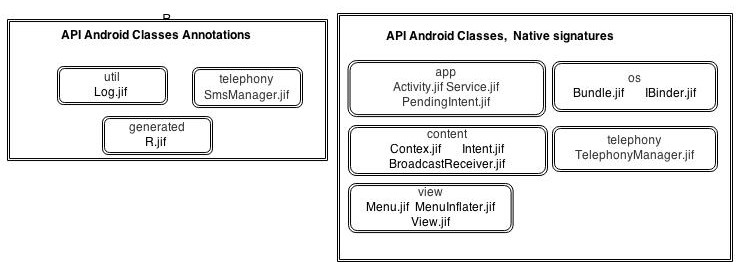
\includegraphics[width=14cm]{desingSol-step1-details.jpg}
	\end{center}
	\caption{Diseño de la solución paso 1. Ilustra las clases especificas de la
	clase de Android, anotadas manualmente.}
	\label{fig:desingSol-step1}
\end{figure}

Paso dos: 
Definir Autoridades y forma de annotación del programa android a analizar.
Una clase Android tendrá una Autoridad máxima(un principal), en este caso Alice,
así que, información con nivel de seguridad alto deberá pertenecer a dicha
autoridad.\newline
Jif hace seguimiento al flujo de información del programa, asociando un label
de seguridad al program counter de cada sentencia y expresion del programa,
program counter(pc) label. Este pc se ve afectado por el label
de seguridad que se especifique en la declaración de variables y
métodos.\newline 
La sintaxis para anotación de variables es: \newline 
\emph{ type\{L\} varName; } \newline donde type especifíca el tipo de dato que
almacena la variable, \{L\} el label de seguridad  para especificar quien es el
dueño de la variable, y name, el respectivo nombre de la variable.\newline 
Un método se escribe de la forma:\newline
\emph{ type \{RTL\} methodName \{BL\} (arg1\{AL\},,, argn\{AL\}) :\{EL\}
}\newline RTL, Return Type Label, indica el label de seguridad con que
queda el tipo de dato devuelto por el método.\newline 
BL begin label, representa el máximo nivel se seguridad del pc label desde donde
se invoca el método, de este modo, el program counter label desde donde
se invoca el método debe ser menor o igual de restrictivo que el BL del
método.\newline 
AL argument label, indica el máximo nivel de seguridad de los argumentos con que
se invoca el método, así, los labels de los argumentos con que se invoca el
método deben ser menor o igual de restrictivos que los AL con que han
definido el método.\newline
EL end label, indica el pc label en el punto de terminación del método, y
representa la información que puede ser conocida.\newline
Cuando un label no es específicado, Jif define unos por defecto. En el caso de
RTL, jif hace un join entre los diferentes AL con que ha sido definido el
método.\newline

Partiendo de que Jif se fundamenta en labels de seguridad para hacer seguimiento
al flujo de información del programa, es necesario definir los labels a
anotar para métodos y variables del programa.\newline
En el caso de variables con nivel de seguridad  alto, la anotación debe
ser:\newline
\emph{ type\{Alice:\} varName; }\newline
Para el resto de variables, entran a jugar las anotaciones definidas por Jif
acorde al contexto donde están definidas.

Ahora en el caso de los métodos, la anotación varía acorde a si el método debe
influenciar(acceder, modificar) o no, información anotada con nivel de seguridad
alto.
Partiendo de lo anterior, se define un algoritmo de anotación que se condensa en
un generador de anotaciones\newline





